%%%%%%%%%%%%%%%%%%%%%%%%%%%%%%%%%%%%%%%%%%%%%%%%
%% Intro to LaTeX and Template for Homework Assignments
%% Quantitative Methods in Political Science
%% University of Mannheim
%% Fall 2018
%%%%%%%%%%%%%%%%%%%%%%%%%%%%%%%%%%%%%%%%%%%%%%%%

% created by Marcel Neunhoeffer & Sebastian Sternberg


% Every .tex file usually consists of four parts.
% 1. Document Class
% 2. Packages
% 3. Header
% 4. Your Document
 
\documentclass[a4paper,12pt]{article} % This defines the style of your paper

%%%%%%%%%%%%%%%%%%%%%%%%%%%%%%%%%%%%%%%%%%%%%%%%
% 2. Packages
%%%%%%%%%%%%%%%%%%%%%%%%%%%%%%%%%%%%%%%%%%%%%%%%

% Packages are libraries of commands that LaTeX can call when compiling the document.
% If the packages we call are not installed yet, TeXworks will ask you to install the necessary packages while compiling.
\usepackage[top = 2.5cm, bottom = 2.5cm, left = 2.5cm, right = 2.5cm]{geometry} %margins
\usepackage[T1]{fontenc}
\usepackage[utf8]{inputenc}
\usepackage{hyperref} %for external links
\usepackage{multirow}
\usepackage{tikz} %for the flow chart
\usetikzlibrary{shapes,arrows}
\usepackage{amsmath} %math package
\usepackage{amsmath, nccmath} %multiple fractions
\usepackage{pgfplots} %plots
\usepackage{pgfplotstable} %to plot from imported text files
\pgfplotsset{compat = newest}
\usepackage{subcaption} %figures with multiple captions
\usepackage{multirow} % Multirow is for tables with multiple rows within one cell.
\usepackage{booktabs} % For even nicer tables.
\usepackage{graphicx} %to include some plots (.pdf files) we need a package for that.
\usepackage[justification=centering]{caption} %Centering captions under the figures
\usepackage{setspace}
\setlength{\parindent}{0in} %The following command sets the indent to 0.
\usepackage{float} % Package to place figures where you want them.
\usepackage{fancyhdr} % to create nice headers.
\usepackage[numbered, framed]{mcode} %Package for Matlab code listings:
\lstset{stepnumber  = 5, % Line numbers go in steps of 4
	breaklines  = true,
	breakautoindent=true, 
	breakindent=10pt,
	breakatwhitespace   = false,
	prebreak= \space,
	postbreak   = \space}

\newcommand{\tagg}[1]{%
	\tikz[baseline]\node[anchor=base,
	draw=gray!30,
	rounded corners,
	inner xsep=1ex,
	inner ysep =0.75ex,
	text height=1.5ex,
	text depth=.25ex]{#1};
  }

%pgfplots style list (color and style of the plots for each farmer)
\definecolor{farmer1}{HTML}{f28d11} %orange
\definecolor{farmer2}{HTML}{0e5de8} %blue
\definecolor{farmer3}{HTML}{2bd941} %green
\definecolor{farmer4}{HTML}{d41717} %red
\definecolor{crop1}{HTML}{e41a1c} %
\definecolor{crop2}{HTML}{377eb8} %
\definecolor{crop3}{HTML}{4daf4a} %
\definecolor{crop4}{HTML}{984ea3} %
\pgfplotscreateplotcyclelist{farmerslist}{
%Farmer 1
farmer1,every mark/.append style={farmer1},mark=triangle*\\
%Farmer 2
farmer2,every mark/.append style={farmer2},mark=diamond*\\
%Farmer 3
farmer3,every mark/.append style={farmer3},mark=otimes\\
%Farmer 4
farmer4,every mark/.append style={farmer4},mark=star\\
%etc...
}
\pgfplotscreateplotcyclelist{cropslist}{
crop1, thick, every mark/.append style={crop1}, mark=triangle\\
crop2,every mark/.append style={crop2},mark=diamond\\
crop3,every mark/.append style={crop3},mark=otimes\\
crop4, densely dashed,every mark/.append style={crop4},mark=square*\\
%etc...
}


%%%%%%%%%%%%%%%%%%%%%%%%%%%%%%%%%%%%%%%%%%%%%%%%
% 3. Header (and Footer)
%%%%%%%%%%%%%%%%%%%%%%%%%%%%%%%%%%%%%%%%%%%%%%%%
\pagestyle{fancy} % % To make our document nice we want a header and number the pages in the footer. With this command we can customize the header style.
\fancyhf{} % This makes sure we do not have other information in our header or footer.
\lhead{\footnotesize Crop Wars}% \lhead puts text in the top left corner. \footnotesize sets our font to a smaller size. \rhead works just like \lhead (you can also use \chead)
\rhead{\footnotesize Golling, Mourouga, Moser, Schmidt, Keshavarzzadeh} %<---- Fill in your lastnames.
\cfoot{\footnotesize \thepage} % We want to put our page number in the center.

%%%%%%%%%%%%%%%%%%%%%%%%%%%%%%%%%%%%%%%%%%%%%%%%
% 4. document
%%%%%%%%%%%%%%%%%%%%%%%%%%%%%%%%%%%%%%%%%%%%%%%%

\begin{document}

\thispagestyle{empty}
\begin{tabular}{p{15.5cm}}
%---------
{\bf Complex Social Systems: Modeling Agents, Learning, and Games} \\
851-0101-86L, Fall 2021  \\
\hline \\
\end{tabular}
%--------------
\vspace*{0.3cm}
%----------------------------Title
\begin{center}
	{\Large \bf Coding Project: Crop Wars}
	\vspace{2mm}
        
	% YOUR NAMES GO HERE
	{\bf Christopher Golling, Gael Mourouga, Aaron Moser, Otto Schmidt, Amirhassan Keshavarzzadeh }
		
\end{center}  
%-----------------------------
%%%%%%%%%%%%%%%%%%%%%%%%%%%%%%%%%%%%%%%%%%%%%%%%
%%%%%%%%%%%%%%%%%%%%%%%%%%%%%%%%%%%%%%%%%%%%%%%%

\vspace{0.4cm}

%----------------First section
\section{Introduction}

Agricultural structures are shaped by a variety of factors, including economic, environmental, cultural, technological and geographical conditions \cite{happeAgriculturalPoliciesFarm2004}. \\
Consequently, both farmers and policymakers can benefit from farm-level models which optimise water usage and crop nature, based on a set of different externalities including water resources availability and market dynamics.\\
The model featured in this coding project aims to illustrate the process behind the development of agent-based farm-level models, by starting with a simple, deterministic model that is progressively complexified with elements from physics-based models, game theory and reinforcement learning.


\section{State-of-the-Art}

To guide the development of our illustrative model, a literature review was conducted to assess the state-of-the-art on agent-based modelling for water resources allocation and farming simulations. \\
Our starting point was the thesis \textit{"Agricultural policies and farm structures: Agent-based modelling and application to EU-policy reform"} by Happe (2004) \cite{happeAgriculturalPoliciesFarm2004}, which outlines in details the development of an agent-based model (AgriPoliS) to assess the influence of agricultural policies at the farm level, which is applied to a case study in the region of Holenhole in Germany.\\
To have an overview of more recent approaches. a seed review paper was selected, \textit{"A review of Agent Based Modeling for agricultural policy evaluation"} by Kremmydas et al.(2018) \cite{kremmydasReviewAgentBased2018} from which a literature graph was generated using the online tools \href{https://www.connectedpapers.com/main/35fac7b643317e5f48f5280fadec94051bf2401f/A-review-of-Agent-Based-Modeling-for-agricultural-policy-evaluation/graph}{Connected Papers}, and is analysed on figure \ref{State_of_the_art}.\\
For completeness, the graphs generated through other seed papers were also analysed, including an older paper applying game theory to decision making in farmer cooperatives by Staatz (1983) \cite{staatzGametheoreticAnalysisDecision1983} and a case application of agent-based models to water allocation on the transboundary Nile river by Ding (2016) \cite{dingAgentBasedModelling2016}.\\
One thing which became apparent through our literature review was that the parametrisation of the models with real-life data, calibration and sensitivity analysis, as well as the model validation through the analysis of existing agricultural systems was the most time and ressource-consuming part of the studies. As such, we decided to procedurally generate data related to externalities (crop price and availability, weather data, water resources availability) and to generate a virtual geography for our agent-based model, centering our study around the construction of the model itself and the analysis of the interactions between agents for a given set of externalities.



\begin{figure}[tb]
	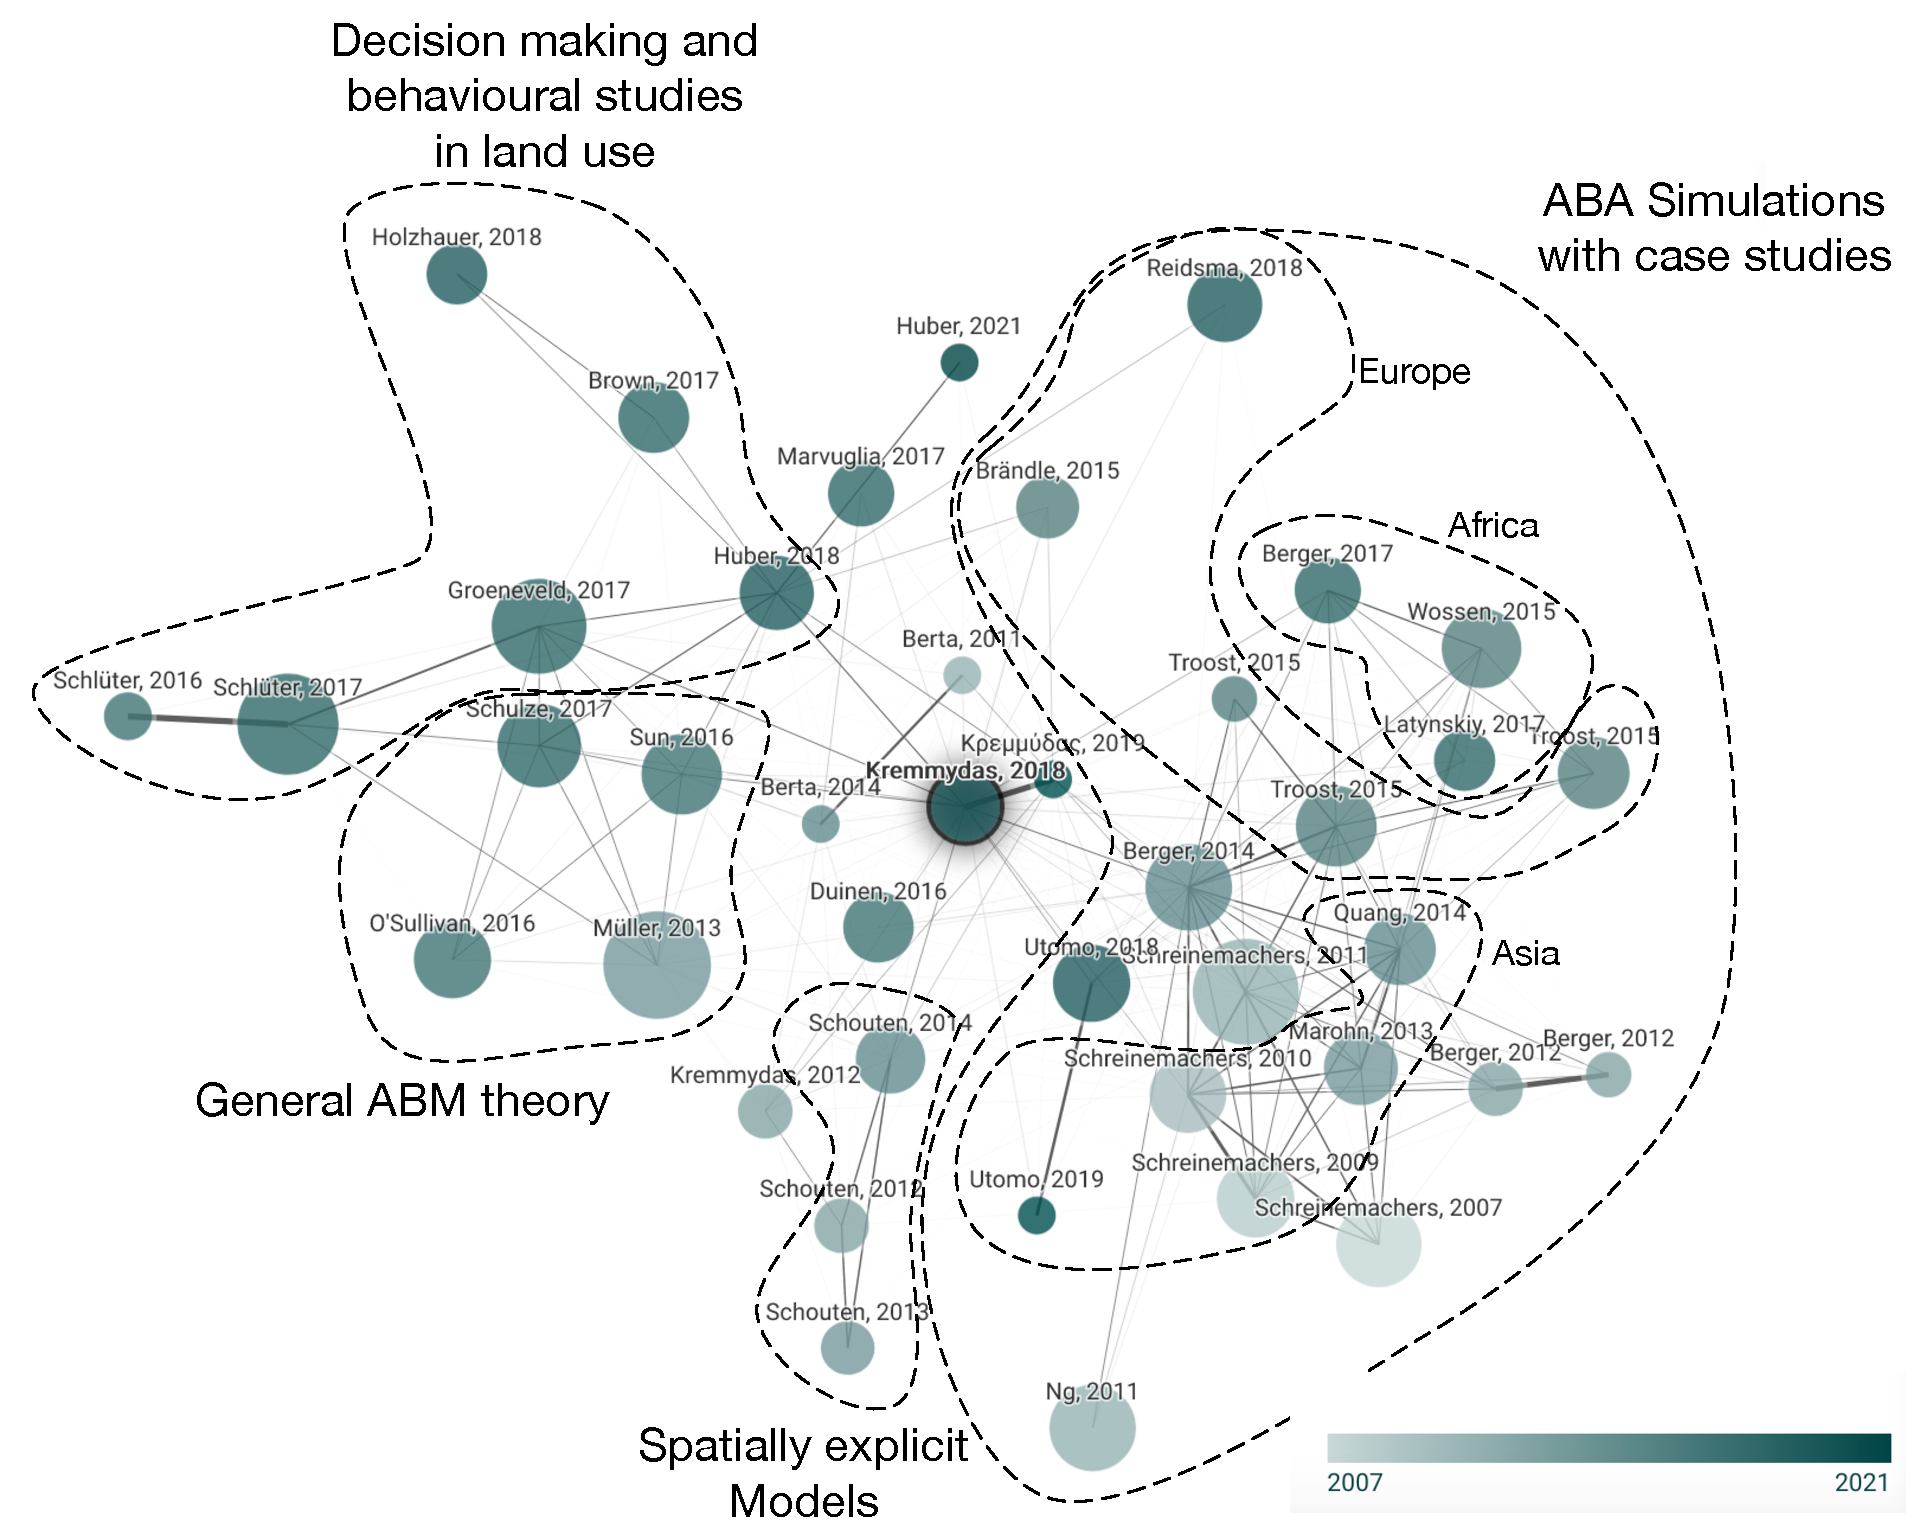
\includegraphics[width=.8\textwidth]{Figures/StateOfTheArt2.pdf}
	\centering
	\caption{\small Graph showing papers related to ref. \cite{kremmydasReviewAgentBased2018} generated on \href{https://www.connectedpapers.com/main/35fac7b643317e5f48f5280fadec94051bf2401f/A-review-of-Agent-Based-Modeling-for-agricultural-policy-evaluation/graph}{Connected Papers}. Circle radius is proportional to number of citation, color to publication date, dashed line refers to paper categories. ABM: agent-based modelling, ABA: agent-based agricultural simulations.}
	\label{State_of_the_art}
\end{figure}

\section{The Crop War model}

\subsection{Concept}
The Crop War model aims to visualise how farmers can compete with respect to water resources and crop profitability, given a geographical environment (procedurally generated) and a set of externalities including market dynamics (supply and demand impacting the price of crops), agent personalities and weather conditions.

\subsection{Overview} \label{overview}
In order to illustrate the development of our Crop Wars model, we organised the model in versions, starting from purely deterministic models with added layers of complexity, on top of which we implemented Reinforcement Learning (RL) to identify the best strategies for a given set of externalities and a specific reward function.

In \tagg{v1.1}, the model is not spatially resolved, in the sense that each agent has a single cell (farm) on which it can grow a single crop (out of four different crops) and at each time step decides to sell or stock its yield.

In \tagg{v1.2} we implement the \href{https://n.ethz.ch/~cgolling/gess/html/VIS_map.html}{\texttt{Map}} class and the possibility for spatial expansion, where agents can buy neighbouring cells in order to grow more crops.

In \tagg{v1.3}, we implement a \href{https://n.ethz.ch/~cgolling/gess/html/INFO_market.html}{\texttt{Market}} model, where the total amount of a given produced crop impacts its price, given a certain demand.

The market also incorporates agent personalities, where different personalities may have different tendencies to expand spatially or sell and/or stock commodities.

These deterministic versions pave the way to the Reinforcement Learning (RL) model, which is implemented in \tagg{v2}. In \tagg{v2.1}, a RL agent will play against an expanding agent (i.e. \href{https://n.ethz.ch/~cgolling/gess/html/code/agents.html#agents.Introvert}{\texttt{Introvert}}, see section \ref{sec:v13}). The reward function, which the RL agent tries to maximize, is the budget evolution. In the next version \tagg{v2.2}, the RL agent will compete against the \href{https://n.ethz.ch/~cgolling/gess/html/code/agents.html#agents.Trader}{\texttt{Trader}} agent (see sec. \ref{sec:v13}). In this version, both spatial expansion and market decision play a role.

\begin{figure}[H]
	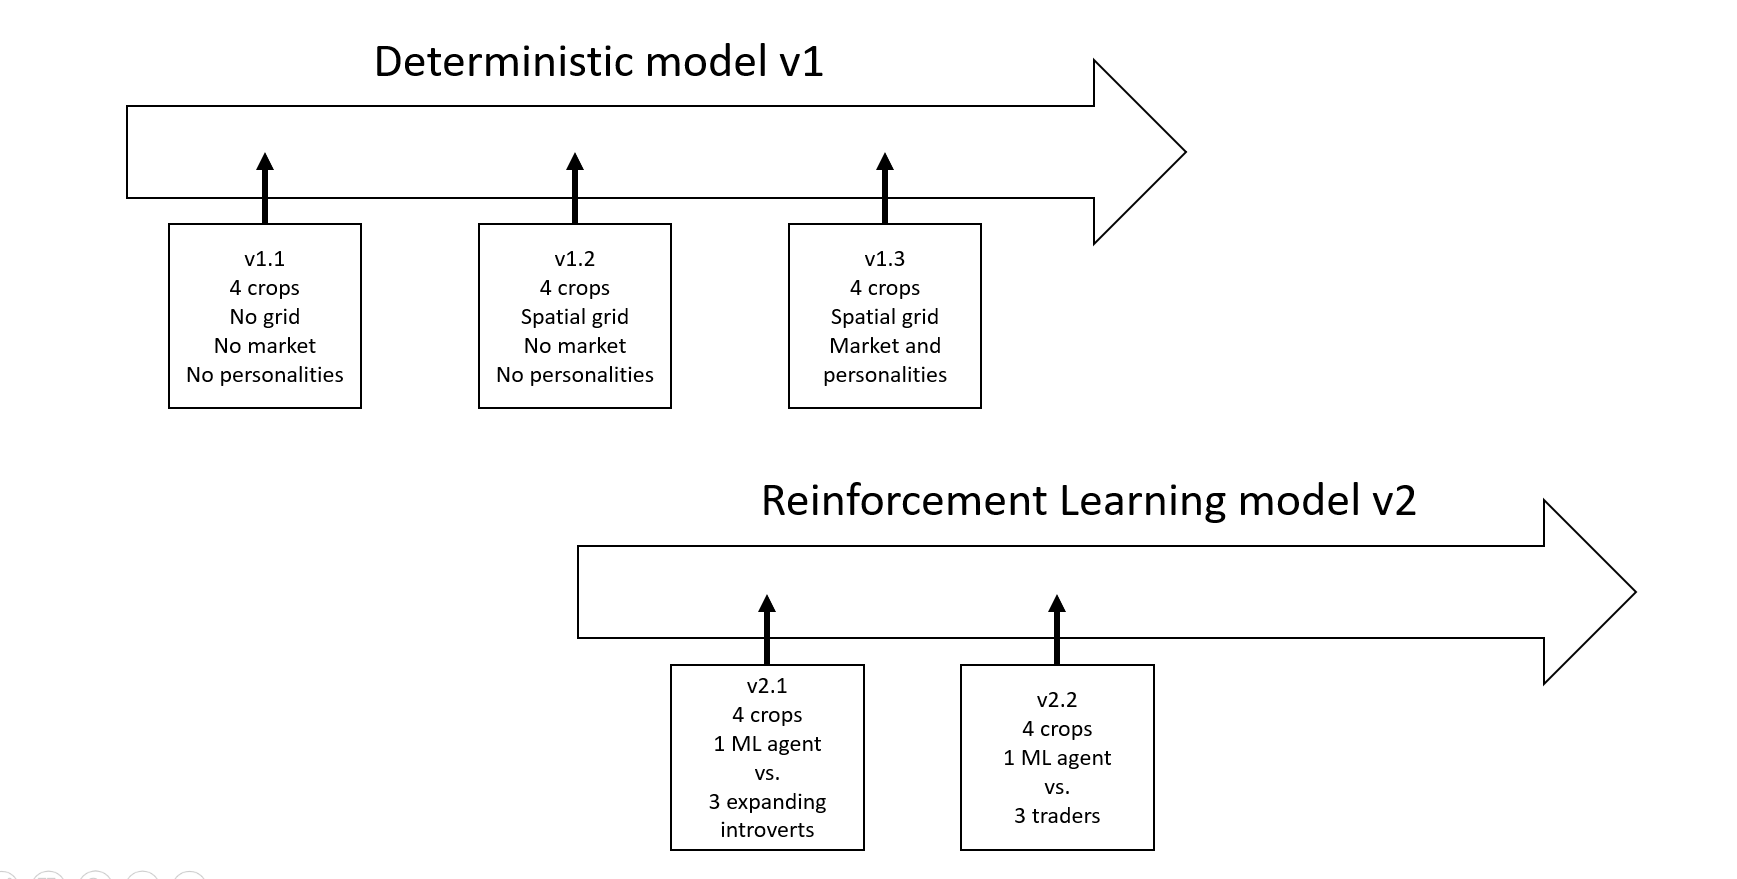
\includegraphics[width=\textwidth]{Figures/version design.PNG}
	\centering
	\caption{\small Overview of the different model versions}
	\label{fig:Overview}
\end{figure}

\subsection{Software}
In order to build the model, we decided to use the python library \href{https://agentpy.readthedocs.io/en/stable/overview.html}{\texttt{agentpy}} which conveniently introduces the \texttt{Agent}, \texttt{Grid}, \texttt{Model}, and \texttt{Experiment} classes, allowing to create our model with minimal prerequisite work. A \href{https://n.ethz.ch/~cgolling/gess/html/index.html}{documentation} of the CropWar model was created, to define functions and variables, and make the code more readable. Verbatim text indicates used function or classes. Exact and extensive descriptions of these objects can then be found in this documentation.

All relevant programs and files were hosted on a \href{https://github.com/Anon75014/AgentBasedModelling}{GitHub repository}, with which our team interacted using Visual Studio Code and GitHub Desktop to navigate between different model versions (hosted on different branches of the GitHub tree).The report and presentation were generated via LaTeX and hosted on the \href{https://github.com/Anon75014/AgentBasedModelling}{GitHub repository}.

\subsubsection{Team members and workflow}

The Python developers were Christopher Golling and Aaron Moser, who implemented the first iterations of the deterministic model, before Aaron focused on the market and personalities, while Christopher started working on the Reinforcement Learning model.

Otto Schmidt and Ga\"el Mourouga designed the market model and tested the code in order to issue the best values for each parameters. They were also in charge of the report and the presentation, and were the main LaTeX developers.

Otto and Christopher also created the \href{https://n.ethz.ch/~cgolling/gess/html/index.html}{documentation}, in order to make code review and future usage easier.

Amirhassan Keshavarzzadeh proposed the idea of a project revolving around water ressources and farming, and was in charge of the \texttt{crops.py} file and the FAO model, where realistic values for the seed costs and yields would have been entered and implemented in the Crop Wars model.



%At each time step $dt$, all agents collect their crop yields and are faced with the choice of selling it at market price or stocking it for later use. Agents can also change the crops they are growing, or leave their land idle for replenishment of its nutritive properties, where the respective probabilities of these choices can be influenced by agent personalities.\\
%The wealth $W_i$ of each agent is then plotted as a function of time $t$, and an analyis is carried out to explain the success rate of different strategies, given a set of externalities such as weather conditions or government policies.


\subsection{Deterministic model development}

\subsubsection{Crop factors}
In the current model, four different crops (winter wheat, barley, maize, beans) have been considered for agents to choose from. 
% Maize and beans are more water stress-resistant than winter wheat and barley. This variation in water stress resistivity can make the agent’s competition more severe. On the other hand, the more water-resistant crops have less harvest yield and price, therefore less revenue per unit area. 
% Therefore, by choosing this combination of crops there will be a tradeoff between revenue and availability of resources (capital cost, water). 
The property of each crop can be defined by four values: seed cost, sell price, maximum harvest yield and water consumption. Seed costs and sell prices are factors which determine the total revenue \cite{Jose}. 


Maximum harvest yield is an important factor that is used to calculate the actual crop’s harvest yield.  The maximum harvest yield is based on empirical data under different climate conditions. For winter wheat, barley, maize, and beans the maximum harvest yields are obtained from \cite{w9030157}. Water consumption illustrates how each stage of crop development will decrease under the water stress situation \cite{VAUX198361}.

These factors were initialized for the model in \href{https://n.ethz.ch/~cgolling/gess/html/code/crops.html}{\texttt{crop}} module.

The crops will be numbered throughout the report as follows:
\begin{center}
\begin{tabular}{ ||c|c|| } 
\hline
Crop & Crop ID  \\
\hline
Winter wheat & 1\\
Barley & 2 \\
Maize & 3 \\
Beans & 4 \\
\hline
\end{tabular}
\end{center}


% crop development stages are vegetative stage, stem elongation stage, booting stage, heading stage, anthesis stage, milking stage, dough stage, ripe seed stage. Ky is empirically obtained and for the present study, the values of Ky are adopted from the FAO report \cite{Najarchi2011DeterminationOT}. Crop factor is another important factor that development stages time for each crop. The crop factor is empirically determined \cite{UCAN2007249}. Crop factors can consider how much different development stages of crops are vulnerable to water stress. These factors can be used in the FAO model to determine the actual harvest yield and therefore the realistic agricultural revenue. 
These coefficients will be used in the FAO model \cite{allenFAO24Reference1991} as follows :

\begin{equation}\label{eq:harvest_yield}
    1-\frac{Y_t}{Y^{m}} = \sum_{i=1}^{n} k_{y,i} \cdot(1-\frac{d_{i,t}}{ET_{m,i}}) 
\end{equation}

\begin{equation}
    ET_{m.i}=k_{c.i} \cdot ET_o 
\end{equation}
Here $Y_t$ is the crop harvest yield in tons per ha per time step, $Y^m$ is the maximal crop harvest yield in tons per ha, $k_{y,i}$ are empirical non-dimensional values relating water stress to crop yield. The \(ET_o\) is the reference evapotranspiration, it considers the effects of the climate on the crop evapotranspiration and is set to $1.0$ to reduce the modelling effort. Finally $d_{i,t}$ is the water availability in each time step and $k_{c,i}$ is the crop factor.

The formula~\eqref{eq:harvest_yield} is used in order to calculate the harvest yield for each crop in the following model.

\subsubsection{Version 1.1}
The first version of the model \tagg{v1.1} is not spatially resolved, in the sense that each agent can only grow one crop at a time and can not expand to other locations.

The price of each crop is fixed and does not vary as a function of time, and the agents only have the choice between selling or stocking their yields, their storage space being unlimited. Fig.(\ref{Graphv11}) show the evolution of the budget (in \$) and stock as a function of time over 10 time steps for 5 agents choosing between 2 crops to grow:


\pgfplotstableread[col sep=comma]{Data/v11_exported_budget.csv}{\budgeta}
\pgfplotstableread[col sep=comma, skip first n=3]{Data/v11_exported_stock.csv}{\stocka}


%figure showing 4 subfigures: wealth, crop stocks (1 and 2) and the map
\begin{figure}[H]
	%wealth
\begin{subfigure}[hb]{0.45\textwidth}
	\resizebox{\linewidth}{!}{
		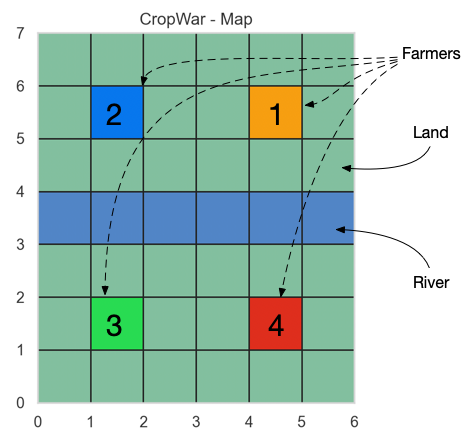
\includegraphics[width=\textwidth]{Figures/v11_Map.png}
	}
\end{subfigure}
\hfill
%crop 1
\begin{subfigure}[hb]{0.5\textwidth}
	\resizebox{\linewidth}{!}{\begin{tikzpicture}
		\pgfplotsset{
			scale only axis,
		}
		%axis options:
		\begin{axis}[
		  xlabel=Time step (years),
		  ylabel=Farmer wealth (\$),
		  xmin=0,
		  %ymin=350,
		  legend pos=north west,
		  cycle list name=farmerslist
		]
		  %plot 1: farmer ID 1
		  \addplot+[] table[y index =1]{\budgeta};
		  \addlegendentry{$1$}
		  
		  %plot 2: farmer ID 2
		  \addplot+[]  table[y index =2]{\budgeta};
		  \addlegendentry{$2$}
  
		  %plot 3: farmer ID 3
		  \addplot+[] table[y index =3]{\budgeta};
		  \addlegendentry{$3$}
  
		  %plot 4: farmer ID 4
		  \addplot+[] table[y index =4]{\budgeta};
		  \addlegendentry{$4$}
  
		\end{axis}
	  \end{tikzpicture}
	  }
\end{subfigure}
\newline
%crop 1
\begin{subfigure}[hb]{0.5\textwidth}
	\resizebox{\linewidth}{!}{\begin{tikzpicture}
		\pgfplotsset{
			scale only axis,
		}
	  
		\begin{axis}[
		  xlabel=Time step (years),
		  ylabel=Farmer stock of crop A,
		  xmin=0,
		  ymin=0,
		  legend pos=north west,
		  cycle list name=farmerslist
		]
		  %plot 1: farmer ID 1
	  \addplot+[] table[y index =1]{\stocka};
	  \addlegendentry{$1$}
	  
	  %plot 2: farmer ID 2
	  \addplot+[]  table[y index =2]{\stocka};
	  \addlegendentry{$2$}

	  %plot 3: farmer ID 3
	  \addplot+[] table[y index =3]{\stocka};
	  \addlegendentry{$3$}

	  %plot 4: farmer ID 4
	  \addplot+[] table[y index =4]{\stocka};
	  \addlegendentry{$4$}

	  \end{axis}
	  \end{tikzpicture}
  }
\end{subfigure}
\begin{subfigure}[hb]{0.5\textwidth}
	\resizebox{\linewidth}{!}{\begin{tikzpicture}
		\pgfplotsset{
			scale only axis,
		}
	  
		\begin{axis}[
		  xlabel=Time step (years),
		  ylabel=Farmer stock of crop B,
		  xmin=0,
		  ymin=0,
		  legend pos=north west,
		  cycle list name=farmerslist
		]

		  \addplot table[y index =5]{\stocka};
		  \addlegendentry{$1$}
		  \addplot table[y index =6]{\stocka};
		  \addlegendentry{$2$}
		  \addplot table[y index =7]{\stocka};
		  \addlegendentry{$3$}
		  \addplot table[y index =8]{\stocka};
		  \addlegendentry{$4$}
		\end{axis}
	  \end{tikzpicture}
  }
\end{subfigure}
\caption{Graph showing the map with four farmers (denoted 1,2,3 and 4), the evolution of crop stocks the and farmer's budget as a function of time over 10 time steps}
\label{Graphv11}
\end{figure}

\subsubsection{Version 1.2}
In the second version of the model \tagg{v1.2}, \href{https://n.ethz.ch/~cgolling/gess/html/VIS_map.html}{\texttt{Map}} class was created, so that agents can expand their farms in order to grow more crops. A \texttt{buy\_cell\_threshold} between 0 and 1 is defined for each agent, representing the tendency of agents to expand their farms (0 corresponding to agents expanding as much as possible, and 1 to agents remaining on their initial cell).
\begin{figure}[H]
	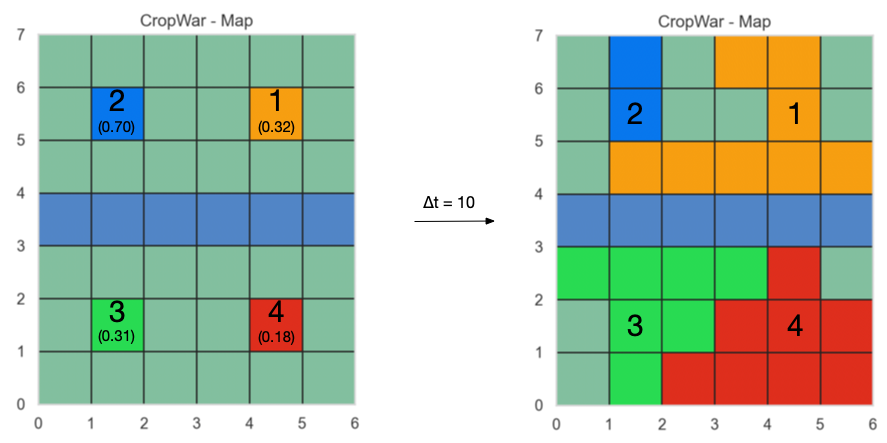
\includegraphics[width=.8\textwidth]{Figures/v12_Map.png}
	\centering
	\caption{\small Evolution of farmers' land count on the grid over 10 time steps. Number in brackets indicate the farmer's \texttt{buy\_cell\_threshold}}
	\label{Mapv12}
\end{figure}


%run SEED: b'G\x11\xd9\xec0H\xfb\x83n\n' on 30.11.2021 at 4pm
\pgfplotstableread[col sep=comma]{Data/v12_exported_budget.csv}{\budgetb}
\pgfplotstableread[col sep=comma, skip first n=3]{Data/v12_exported_stock.csv}{\stockb}
\pgfplotstableread[col sep=comma, skip first n=1]{Data/v12_exported_cellcount.csv}{\cellcountb}

%figure showing 4 subfigures for v12: wealth, crop stocks (1 and 2) and the map
\begin{figure}[H]
	%wealth
\begin{subfigure}[hb]{0.48\textwidth}
	\resizebox{\linewidth}{!}{\begin{tikzpicture}
		\pgfplotsset{
			scale only axis,
		}
		%axis options:
		\begin{axis}[
		  xlabel=Time step (years),
		  ylabel=Farmer land count (cells),
		  xmin=0,
		  legend pos=north west,
		  cycle list name=farmerslist
		]
		  %plot 1: farmer ID 1
		  \addplot+[] 
			  table[y index =1]{\cellcountb};
		  \addlegendentry{$1$}
		  
		  %plot 2: farmer ID 2
		  \addplot+[]  table[y index =2]{\cellcountb};
		  \addlegendentry{$2$}
  
		  %plot 3: farmer ID 3
		  \addplot+[] table[y index =3]{\cellcountb};
		  \addlegendentry{$3$}
  
		  %plot 4: farmer ID 4
		  \addplot+[] table[y index =4]{\cellcountb};
		  \addlegendentry{$4$}
  
		\end{axis}
	  \end{tikzpicture}
	}
\end{subfigure}
\hfill
%crop 1
\begin{subfigure}[hb]{0.5\textwidth}
	\resizebox{\linewidth}{!}{\begin{tikzpicture}
		\pgfplotsset{
			scale only axis,
		}
		%axis options:
		\begin{axis}[
		  xlabel=Time step (years),
		  ylabel=Farmer wealth (\$),
		  xmin=0,
		  ymax = 600,
		  legend pos=north west,
		  cycle list name=farmerslist
		]
		  %plot 1: farmer ID 1
		  \addplot+[] 
			  table[y index =1]{\budgetb};
		  \addlegendentry{$1$}
		  
		  %plot 2: farmer ID 2
		  \addplot+[]  table[y index =2]{\budgetb};
		  \addlegendentry{$2$}
  
		  %plot 3: farmer ID 3
		  \addplot+[] table[y index =3]{\budgetb};
		  \addlegendentry{$3$}
  
		  %plot 4: farmer ID 4
		  \addplot+[] table[y index =4]{\budgetb};
		  \addlegendentry{$4$}
  
		\end{axis}
	  \end{tikzpicture}
	  }
\end{subfigure}
\newline
%crop 1
\begin{subfigure}[hb]{0.5\textwidth}
	\resizebox{\linewidth}{!}{\begin{tikzpicture}
		\pgfplotsset{
			scale only axis,
		}
	  
		\begin{axis}[
		  xlabel=Time step (years),
		  ylabel=Farmer stock of crop A,
		  xmin=0,
		  ymin=0,
		  legend pos=north west,
		  cycle list name=farmerslist
		]
		  %plot 1: farmer ID 1
	  \addplot+[] table[y index =1]{\stockb};
	  \addlegendentry{$1$}
	  
	  %plot 2: farmer ID 2
	  \addplot+[]  table[y index =2]{\stockb};
	  \addlegendentry{$2$}

	  %plot 3: farmer ID 3
	  \addplot+[] table[y index =3]{\stockb};
	  \addlegendentry{$3$}

	  %plot 4: farmer ID 4
	  \addplot+[] table[y index =4]{\stockb};
	  \addlegendentry{$4$}

	  \end{axis}
	  \end{tikzpicture}
  }
\end{subfigure}
\begin{subfigure}[hb]{0.5\textwidth}
	\resizebox{\linewidth}{!}{\begin{tikzpicture}
		\pgfplotsset{
			scale only axis,
		}
	  
		\begin{axis}[
		  xlabel=Time step (years),
		  ylabel=Farmer stock of crop B,
		  xmin=0,
		  ymin=0,
		  legend pos=north west,
		  cycle list name=farmerslist
		]

		  \addplot+[] table[y index =5]{\stockb};
		  \addlegendentry{$1$}
		  \addplot+[] table[y index =6]{\stockb};
		  \addlegendentry{$2$}
		  \addplot+[] table[y index =7]{\stockb};
		  \addlegendentry{$3$}
		  \addplot+[] table[y index =8]{\stockb};
		  \addlegendentry{$4$}
		\end{axis}
	  \end{tikzpicture}
  }
\end{subfigure}
\caption{Graph showing the farmer's land count, the evolution of crop stocks and the farmer's budget as a function of time over 10 time steps}
\end{figure}


\newpage
\subsubsection{Version 1.3} \label{sec:v13}
Once the fundamental properties of the model and the \texttt{Map} class were defined , the second interaction platform, i.e. the \href{https://n.ethz.ch/~cgolling/gess/html/INFO_market.html}{\texttt{Market}} model, was implemented in \tagg{v1.3}. In this model, prices aggregate globally.

%\\~\\
% The linear supply of an agent $i$ for a commodity $j$ reads:
% \begin{equation}
%     S_i(p_j) = A + c_i p_j
% \end{equation}
% where $A$ is a surplus supply (willingness to supply for $p_j=0$), $p_j$ the global commodity price and $c_i$ the slope of supply (which is connected to the inverse price elasticity of supply).
% \paragraph{Commodity demand}
% %\\~\\
% The linear demand for a commodity $j$ is globally defined as:
% \begin{equation}
%     D_j(p_j) = d_j \cdot \left( B(p_j) + \delta \right)
% \end{equation}
% where $B(p_j)$ is a baseline demand, $d_j$ a demand shift and $\delta \in [0,1]$ a random variable. 
% \\
% Since the market, i.e. the stock and supply of the agents, expands, the baseline demand $B(p_j) = B + a \cdot S(p_j)$ needs to increase proportionally to account for the expanding market. In each iteration the initial baseline $B$ is increase by a fraction $a$ of the global supply $S(p_j)$.\\
% Another underlying assumption of this version is symmetric information for all market participants. This is important in price aggregation: if all agents know the other agents stocks, they can anticipate the market price. This is implemented in \texttt{Market} by making each agents stock a global variable.
% \\
% For the \href{https://n.ethz.ch/~cgolling/gess/html/code/agents.html}{}\texttt{Trader} agent class we can observe the market interaction by tracing the crop choices of each agent. Fig. \ref{fig:crop choice} shows the crop choices for one representative \texttt{Trader} agent.
% \begin{figure}[H]
%     \centering
%     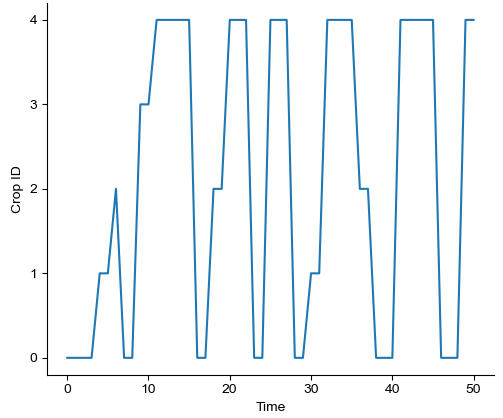
\includegraphics[width = 0.6\textwidth]{Report/Figures/crop choices.PNG}
%     \caption{Cultivated crops for a market interactive agent as a function of time. Here Crop ID from 0 to 4 represents the different commodities in the market.}
%     \label{fig:crop choice}
% \end{figure}
\paragraph{Commodity demand}
From \cite{zulfiqarDevelopmentSupplyDemand2010} in agriculture the demand is usually a strong function of the population to feed, and a weak function of the price.

We therefore define the global demand for crop $j$ as follows:
\begin{equation}
    D_j(p_j) = \left( D_0 + at^2 \right) e^{-\alpha (p_j-p_{j0})}
\end{equation}
Where $D_0$ is a base demand, $at^2$ is a term representing population (and demand) growth as a function of time $t$, $p_j$ is the price of crop $j$ at time $t$, $p_{j,0}$ is the base price of crop $j$, and $\alpha$ is a demand slope, representing the fact that less and less people will be able to afford expensive crops.

\paragraph{Commodity demand}
The supply of crop $j$ by farmer $i$ is limited by his stock of this crop $s_j$, plus the yield at time t $Y_j$, but more importantly is a function of the willingness of the agent to supply a crop at a given price:
\begin{equation}
    S_i(p_j) = A + c_i \cdot p_j
\end{equation}
Here $c_i$ is the willingness to supply crop $j$  at a given price $p_j$ by farmer $i$ and $A$ is the surplus or his willingness to supply crops for free.

\paragraph{Price aggregation}
Price of crop $j$ from supply and demand:
\begin{equation}
    p_j =  p_{j,0} \cdot \frac{D_j(p_j)}{K \cdot \sum_i s_j}
\end{equation}
Where $p_{j,0}$ is the base price of commodity $j$, $D_j(p_j)$ the demand and $\sum_i s_j$ the total stock available of crop $j$ across all farmers. The constant $K$ represents a residual stock of a commodity and is equal for all $j$. This constant is implemented for two reasons:
\begin{enumerate}
    \item In a realistic market with a sufficiently large supply side, the global stock of a commodity will not reach zero. We assume that there will always be some residual "reserve" stock. 
    \item If the global stock for a commodity should reach zero, we are confronted with a mathematical singularity. The constant $K$ was incorporated to avoid this inconvenient behaviour. 
\end{enumerate}


\paragraph{Agent strategies}
For now, the performance of all agents only depends on the initial random choice of a position. However, in order to see different outcomes, a set of strategies needs to be defined.

A strategy is defined on an interaction platform. In this model we use two platforms: the market and geographical expansion.

The agents on such platforms can be split into interactive and non-interactive agents (see \href{https://n.ethz.ch/~cgolling/gess/html/code/agents.html}{\texttt{agents}}), i.e. an agent class able to adapt and a baseline class.

For the market platform the strategy types are:
\begin{enumerate}
        \item \href{https://n.ethz.ch/~cgolling/gess/html/code/agents.html#agents.Trader}{\texttt{Trader}}: compares prices of market commodities, i.e. crops, and decides to switch to crop $j$ if the expected profit $P_j$ is bigger than the profit for a crop $i$ before $P_{old,i}$:
        \begin{equation}
            P_j (p_j) = (D_j - s_j) \cdot p_j > P_{old,i}
        \end{equation}
        \item \href{https://n.ethz.ch/~cgolling/gess/html/code/agents.html#agents.Introvert}{\texttt{Introvert}}: baseline agent. No adaption to market prices. The introvert stays with the initial crop choice and supplies a fixed fraction of the stock.
\end{enumerate}

The strategies of the expansion platform are not discrete and defined via specific agents classes. The tendency to expand is given with the fixed value \texttt{buy\_cell\_threshold}. Each  iteration, the agent decides randomly a value $\in[0,1]$. If \texttt{buy\_cell\_threshold} is bigger than this random value, expansion will not take place. Any value between 0 and 1 however makes expansion possible.

\paragraph{Dynamics}

Each iteration of this version can be separated into three steps:
\begin{enumerate}
    \item Harvesting period: agents harvest according to their crop choice and add the harvest yield to the stock. 
    \item Interaction period: market interaction takes place.
    \item Strategy period: the trader type of the farmers will react on market prices and eventually change the crop. Agents can also buy cells (expand) if \texttt{buy\_cell\_threshold} is large enough.
\end{enumerate}

An illustration of this process is given in the graphs below. These show the dynamics of two \texttt{Trader} and two \texttt{Introvert} agents over 50 time steps.

It is important to note that the different strategies lead to different outcomes. Graph \ref{fig:budget evol} shows the budget evolution of the four agents. Here agent 1 and 2 are \texttt{Trader} agents, agent 3 and 4 are \texttt{Introverts}. We can see that over 50 time steps, the \texttt{Trader} class generates more profits. This can be expected since they are able to adapt to market prices and therefore have an advantage.

\newpage
%run SEED: b'G\x11\xd9\xec0H\xfb\x83n\n' on 30.11.2021 at 4pm
\pgfplotstableread[col sep=comma]{Data/v13_exported_budget.csv}{\budgetc}
\pgfplotstableread[col sep=comma, skip first n=3]{Data/v13_exported_stock.csv}{\stockc}
\pgfplotstableread[col sep=comma, skip first n=1]{Data/v13_exported_cellcount.csv}{\cellcountc}
\pgfplotstableread[col sep=comma]{Data/v13_exported_demand.csv}{\demandc}
\pgfplotstableread[col sep=comma]{Data/v13_exported_prices.csv}{\pricesc}
\pgfplotstableread[col sep=comma]{Data/v13_exported_supply.csv}{\supplyc}
\pgfplotstableread[col sep=comma]{Data/v13_exported_global_stock.csv}{\globalstockc}


\begin{figure}[H]
\begin{subfigure}[hb]{0.5\textwidth}
	\resizebox{\linewidth}{!}{\begin{tikzpicture}
		\pgfplotsset{
			scale only axis,
		}
		%axis options:
		\begin{axis}[
		  xlabel=Time step (years),
		  ylabel=Demand for different crops,
		  xmin=0,
		  xmax=30,
		  legend pos=south east,
		  cycle list name=cropslist
		]
		  %plot 1: farmer ID 1
		  \addplot+[] 
			  table[y index =1]{\demandc};
		  \addlegendentry{$1$}
		  
		  %plot 2: farmer ID 2
		  \addplot+[]  table[y index =2]{\demandc};
		  \addlegendentry{$2$}
  
		  %plot 3: farmer ID 3
		  \addplot+[] table[y index =3]{\demandc};
		  \addlegendentry{$3$}
  
		  %plot 4: farmer ID 4
		  \addplot+[] table[y index =4]{\demandc};
		  \addlegendentry{$4$}
  
		\end{axis}
	  \end{tikzpicture}
	}
\end{subfigure}
\hfill
%crop 1
\begin{subfigure}[hb]{0.5\textwidth}
	\resizebox{\linewidth}{!}{\begin{tikzpicture}
		\pgfplotsset{
			scale only axis,
		}
		%axis options:
		\begin{axis}[
		  xlabel=Time step (years),
		  ylabel=Supply for different crops,
		  xmin=0,
		  xmax=30,
		  legend pos=south east,
		  cycle list name=cropslist
		]
		  %plot 1: farmer ID 1
		  \addplot+[] 
			  table[y index =1]{\supplyc};
		  \addlegendentry{$1$}
		  
		  %plot 2: farmer ID 2
		  \addplot+[]  table[y index =2]{\supplyc};
		  \addlegendentry{$2$}
  
		  %plot 3: farmer ID 3
		  \addplot+[] table[y index =3]{\supplyc};
		  \addlegendentry{$3$}
  
		  %plot 4: farmer ID 4
		  \addplot+[] table[y index =4]{\supplyc};
		  \addlegendentry{$4$}
  
		\end{axis}
	  \end{tikzpicture}
	  }
\end{subfigure}
\newline
%crop 1
\begin{subfigure}[hb]{0.5\textwidth}
	\resizebox{\linewidth}{!}{\begin{tikzpicture}
		\pgfplotsset{
			scale only axis,
		}
	  
		\begin{axis}[
		  xlabel=Time step (years),
		  ylabel=Prices of different crops,
		  xmin=0,
		  ymin=0,
		  legend pos=north west,
		  cycle list name=cropslist
		]
		  %plot 1: farmer ID 1
	  \addplot+[] table[y index =1]{\pricesc};
	  \addlegendentry{$1$}
	  
	  %plot 2: farmer ID 2
	  \addplot+[]  table[y index =2]{\pricesc};
	  \addlegendentry{$2$}

	  %plot 3: farmer ID 3
	  \addplot+[] table[y index =3]{\pricesc};
	  \addlegendentry{$3$}

	  %plot 4: farmer ID 4
	  \addplot+[] table[y index =4]{\pricesc};
	  \addlegendentry{$4$}

	  \end{axis}
	  \end{tikzpicture}
  }
\end{subfigure}
\begin{subfigure}[hb]{0.5\textwidth}
	\resizebox{\linewidth}{!}{\begin{tikzpicture}
		\pgfplotsset{
			scale only axis,
		}
	  
		\begin{axis}[
		  xlabel=Time step (years),
		  ylabel=Total stock of different crops,
		  xmin=0,
		  ymin=0,
		  legend pos=north west,
		  cycle list name=cropslist
		]

		  \addplot+[] table[y index =1]{\globalstockc};
		  \addlegendentry{$1$}
		  \addplot+[] table[y index =2]{\globalstockc};
		  \addlegendentry{$2$}
		  \addplot+[] table[y index =3]{\globalstockc};
		  \addlegendentry{$3$}
		  \addplot+[] table[y index =4]{\globalstockc};
		  \addlegendentry{$4$}
		\end{axis}
	  \end{tikzpicture}
  }
\end{subfigure}
\newline
\begin{subfigure}[hb]{0.45\textwidth}
	\resizebox{\linewidth}{!}{
		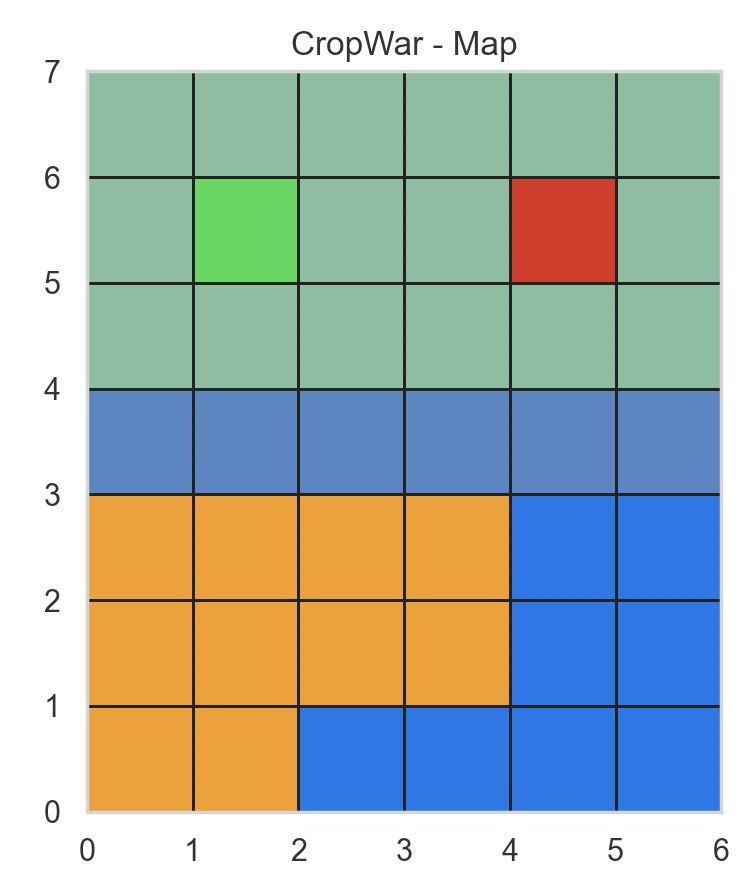
\includegraphics[width=\textwidth]{Figures/v13_Map.png}
	}
\end{subfigure}
\hfill
%crop 1
\begin{subfigure}[hb]{0.5\textwidth}
	\resizebox{\linewidth}{!}{\begin{tikzpicture}
		\pgfplotsset{
			scale only axis,
		}
		%axis options:
		\begin{axis}[
		  xlabel=Time step (years),
		  ylabel=Farmer wealth (\$),
		  xmin=0,
		  %ymin=350,
		  legend pos=north west,
		  cycle list name=farmerslist
		]
		  %plot 1: farmer ID 1
		  \addplot+[] table[y index =1]{\budgetc};
		  \addlegendentry{Trader}
		  
		  %plot 2: farmer ID 2
		  \addplot+[]  table[y index =2]{\budgetc};
		  \addlegendentry{Trader}
  
		  %plot 3: farmer ID 3
		  \addplot+[] table[y index =3]{\budgetc};
		  \addlegendentry{Introvert}
  
		  %plot 4: farmer ID 4
		  \addplot+[] table[y index =4]{\budgetc};
		  \addlegendentry{Introvert}
  
		\end{axis}
	  \end{tikzpicture}
	  }
	 
\end{subfigure}
\caption{Graphs showing the evolution of supply, demand, prices and global stocks for each crop, with the map and the farmer's budget over 50 time steps using the \texttt{Market} model}
\end{figure}
\newpage





\newpage
\subsection{Reinforcement Learning model}

The preceding versions \tagg{v1.1 - v1.3} defined the deterministic agents and the model of the environment in which actions take place. In order to see unpredictable, emerging behaviour, the agents would need to adjust to evolutions of the market and learn. This learning process is modelled via a Reinforcement Learning (RL) as explained in this section. 

Before outlining the technical implementation of the RL approach, a short introduction to RL will be given. 

\subsubsection{Reinforcement Learning}
Within the vast area of machine learning (ML), reinforcement learning describes learning paradigms that focus on optimal decision-making of intelligent agents. 

The decision in RL are modelled with Markov chain processes (MC). The main constituents are the agents, an environment in which the actions take place, states of the agents and an interpreter which determines and interprets the actions of each agent. A schematic of reinforced learning is given in figure \ref{fig:RL schematic}.

\begin{figure}[H]
    \centering
    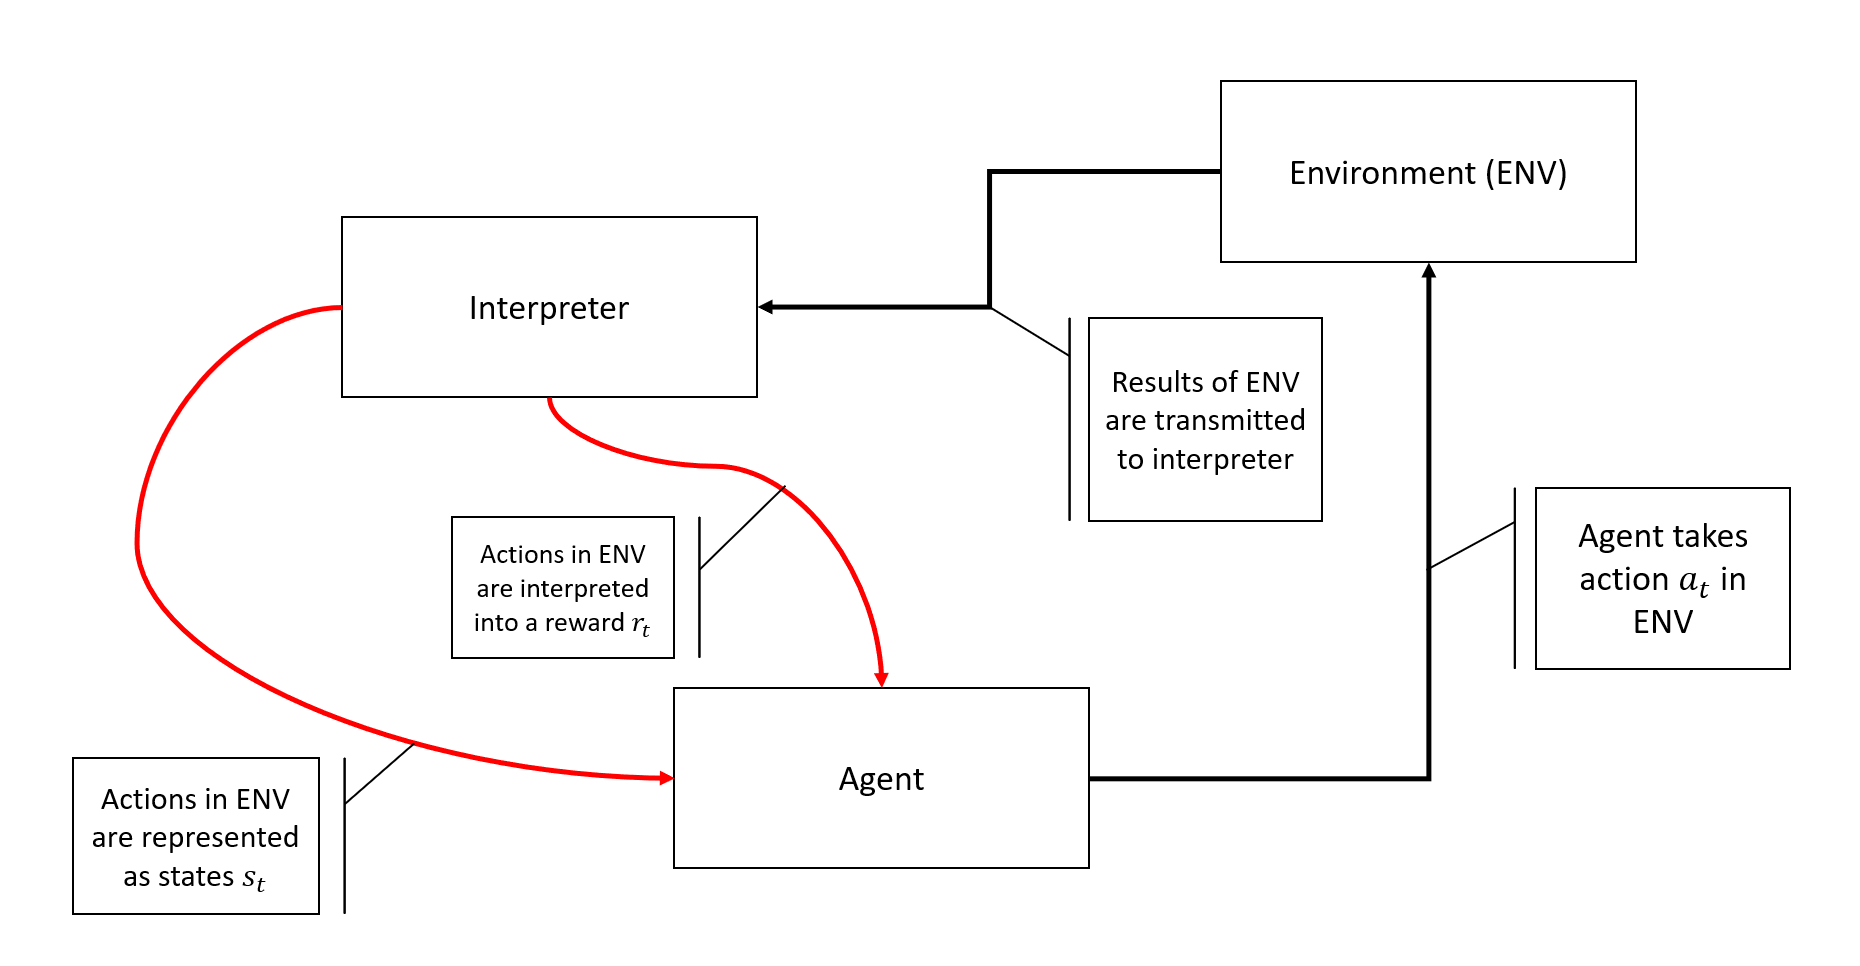
\includegraphics[width = 1\textwidth]{RL schematic.PNG}
    \caption{Feedback loop in RL. An agent decides to do a certain action $a_t$ based on his observation of the environment. This affects the environment, which yields a new state. The effect of the agents' action is then interpreted to update the strategy of the agent.}
    \label{fig:RL schematic}
\end{figure}

The interactions in the above illustrated feedback loop are conducted in discrete iterations or time steps $t$. 
In each iteration, an agent finds itself in a state $s_t$ and with a reward $r_t$. An action $a_t$ is taken in the \href{https://n.ethz.ch/~cgolling/gess/html/INFO_RL_env.html}{environment} from a set of possible actions. The actions lead to results, which are then translated by an \href{https://n.ethz.ch/~cgolling/gess/html/INFO_SB3.html}{interpreter} into a new state and a reward. 
In this process, a RL agent works out a policy $\pi(a_t | s_t)$ after which it will act in a specific environment. This policy is chosen such that the cumulative reward over the iterations is maximal. 

The agent therefore associates certain rewards to a set of actions in combination with their effects at a . In that sense, the agents act according to their associative memory. 

\subsubsection{Proximal Policy Optimization}
There are various ways to implement the schematic RL process of fig. \ref{fig:RL schematic}. In this project, we chose the Proximal Policy Optimization (PPO) algorithm. This is mainly because PPO is suited for environments with discrete time steps, continuous observation space and discrete action space as in our model. The theoretical foundations are given in \cite{schulman2017proximal}. For the software implementation, we follow \cite{stable-baselines3}.

\paragraph{Policy gradient methods}
The PPO algorithm is based on policy gradient methods. Here, the main objective is to compute the gradient of a policy objective and optimize it. 
The policy objective used in \cite{schulman2017proximal} reads

\begin{equation}
    L(\theta) = \hat{\mathbf{E}}_t [log(\pi_{\theta}(a_t|s_t)) \hat{A_t}]
\end{equation}

where:
\begin{enumerate}
    \item $L(\theta)$ - Policy loss function. 
    \item $\pi_{\theta}(a_t|s_t)$ - The stochastic policy in parameter regime $\theta$ given as transition probabilities in the MC of taking action $a_t$ in state $s_t$. It is a neural network, that suggests an action for a given state based on previous training experience.
    \item $\hat{A_t}$ - Estimator of the advantage of the current action. Computed as a discounted reward. This neural net is updated with the experience (i.e. reward) that the agent collects in an environment.
    \item $\hat{\mathbf{E}}_t$ - Expectation for current iteration $t$.
\end{enumerate}

The above function incorporates one main dynamic: if an action $a_t$ resulted in better than average reward during training, the advantage $\hat{A_t}$ will be positive. This yields a positive policy gradient, being defined as the gradient w.r.t. the parameter set $\theta$ (see \cite{schulman2017proximal}):
\begin{equation}
    \hat{g} = \hat{\mathbf{E}}_t [\nabla_{\theta} log(\pi_{\theta}(a_t|s_t)) \hat{A_t}]
\end{equation}

This would increase the probability of taking the same action decision in the same or similar state. Vice versa, the gradient is negative if the advantage is negative, which reduces the probability of taking the corresponding action.

The above defined method is the core technique in PPO of updating policies. However, there are some subtleties which require adjustments. One of which is the Trusted Region Policy Optimization (TRPO) defined in \cite{schulman2017trust}, where unwanted effects of self-reinforced action trajectories can be reduced. 

\paragraph{Implementation}
For the implementation of a PPO model, we used the module 

\href{https://stable-baselines3.readthedocs.io/en/master/index.html}{\texttt{Stable-Baselines3}} (SB3).  Its GitHub repository with all necessary sample functions can be found \href{https://github.com/DLR-RM/stable-baselines3}{here}.
The documentation of the PPO algorithm in this framework can be found \href{https://stable-baselines3.readthedocs.io/en/master/modules/ppo.html}{here}.

As suggested in the documentation of SB3, training was initially performed using the default hyperparameters and the \texttt{MlpPolicy} of SB3. By using \texttt{TensorBoard} to track the learning, we could visually check the agent's performance with the evolution of the mean reward. If no asymptote was reached, the number of steps were increased. By tweaking the learning rate over three orders of magnitudes, we found the default one of 0.0003 to be stable. The number of parallel environments was increased to eight, in order to get a diverse set of initial seeds. This produced high rewards and interesting behaviour.

\newpage

\subsubsection{RL model versions}
As illustrated in fig. \ref{fig:Overview}, we implemented two scenarios. Both differ in the competing benchmark agents. The environment in which the RL agent is trained is defined in section \ref{sec:v13}. The RL agent was trained in this environment in 10000 iterations. The reward function that was used for training is given by
\begin{equation}
    \frac{1}{3}(b^2 + r^2 + s^2)
\end{equation}
where $b$ is the fraction of the global budget that the agent possesses, $r$ is
the current ranking (1 for first, $0.66$ for second, $0.33$ for third, and
$0.0$ for last) and $s$ is the fraction of the global supply that the agent
supplies. It was chosen so to maximize profit of each agent.

\paragraph{Version 2.1}
This version employs the following setup:
\begin{enumerate}
    \item Four crops
    \item Four agents: One ML agent vs. three \texttt{Introvert} agents
\end{enumerate}

The evolution of the budget (i.e. the reward relevant quantity) in this setup is displayed in figure \ref{fig:budget MLvsIntros}.
The trained RL agent generates a higher wealth from the first iteration on. 

\pgfplotstableread[col sep=comma]{Data/MLvsIntroBudget.csv}{\budgetd}

\begin{figure}[H]
    \centering
    {\begin{tikzpicture}
		\pgfplotsset{
			scale only axis,
		}
		%axis options:
		\begin{axis}[
		  xlabel=Time step (years),
		  ylabel=Farmer wealth (\$),
		  xmin=0,
		  %ymin=350,
		  legend pos=north west,
		  cycle list name=farmerslist
		]
		  %plot 1: farmer ID 1
		  \addplot+[thick, no marks] table[y index =1]{\budgetd};
		  \addlegendentry{Introvert}
		  
		  %plot 2: farmer ID 2
		  \addplot+[thick,no marks]  table[y index =2]{\budgetd};
		  \addlegendentry{Introvert}
  
		  %plot 3: farmer ID 3
		  \addplot+[thick,no marks] table[y index =3]{\budgetd};
		  \addlegendentry{RL agent}
  
		  %plot 4: farmer ID 4
		  \addplot+[thick,no marks] table[y index =4]{\budgetd};
		  \addlegendentry{Introvert}
  
		\end{axis}
	  \end{tikzpicture}
	  }
    \caption{Budget evolution over 300 iterations}
    \label{fig:budget MLvsIntros}
\end{figure}


\newpage
\paragraph{Version 2.2}
This version employs the following setup:
\begin{enumerate}
    \item Four crops
    \item Four agents: One ML agent vs. three \texttt{Trader} agents
\end{enumerate}

The three \texttt{Trader} types compete against an RL agent who applies a policy which has been advantageous in 100000 iterations. The budget and cellcount evolution in this setup over 300 iterations is illustrated below.

%seed b'I\x8b\x8f\x8a\x00\xa6\xc9!\xc5 '

\pgfplotstableread[col sep=comma]{Data/MLvsTrader2Budget.csv}{\budgete}

\pgfplotstableread[col sep=comma]{Data/MLvsTrader2Cellcount.csv}{\cellcounte}


\begin{figure}[H]
\begin{subfigure}[hb]{0.5\textwidth}
    \centering
    \resizebox{\linewidth}{!}{\begin{tikzpicture}
		\pgfplotsset{
			scale only axis,
		}
		%axis options:
		\begin{axis}[
		  xlabel=Time step (years),
		  ylabel=Farmer wealth (\$),
		  xmin=0,
		  %ymin=350,
		  legend pos=south west,
		  cycle list name=farmerslist
		]
		  %plot 1: farmer ID 1
		  \addplot+[] table[y index =1]{\budgete};
		  \addlegendentry{Trader}
		  
		  %plot 2: farmer ID 2
		  \addplot+[]  table[y index =2]{\budgete};
		  \addlegendentry{RL agent}
  
		  %plot 3: farmer ID 3
		  \addplot+[] table[y index =3]{\budgete};
		  \addlegendentry{Trader}
  
		  %plot 4: farmer ID 4
		  \addplot+[] table[y index =4]{\budgete};
		  \addlegendentry{Trader}
  
		\end{axis}
	  \end{tikzpicture}
	  }
    \caption{Budget evolution over 300 iterations}
    \label{fig:budget MLvsTraders}
\end{subfigure}
\hfill
\begin{subfigure}[hb]{0.5\textwidth}
    \centering
    \resizebox{\linewidth}{!}{\begin{tikzpicture}
		\pgfplotsset{
			scale only axis,
		}
		%axis options:
		\begin{axis}[
		  xlabel=Time step (years),
		  ylabel=Farmer land count (cells),
		  xmin=0,
		  legend pos=south east,
		  cycle list name=farmerslist
		]
		  %plot 1: farmer ID 1
		  \addplot+[] 
			  table[y index =1]{\cellcounte};
		  \addlegendentry{Trader}
		  
		  %plot 2: farmer ID 2
		  \addplot+[]  table[y index =2]{\cellcounte};
		  \addlegendentry{RL agent}
  
		  %plot 3: farmer ID 3
		  \addplot+[] table[y index =3]{\cellcounte};
		  \addlegendentry{Trader}
  
		  %plot 4: farmer ID 4
		  \addplot+[] table[y index =4]{\cellcounte};
		  \addlegendentry{Trader}
  
		\end{axis}
	  \end{tikzpicture}
	}
    \caption{Cellcount of the agents over 300 iterations}
    \label{fig:cellcount MLvsTraders}
\end{subfigure}
\caption{Budget and cellcount evolution}
\end{figure}

The budget evolution in fig. \ref{fig:budget MLvsTraders} shows how the RL agent generates a higher wealth over 300 iterations compared to the three \texttt{Trader} types as benchmark. Interestingly, from fig. \ref{fig:cellcount MLvsTraders} we can see that the winning strategy does not lead to a high cellcount since the RL agent has the lowest number of cells after all iterations.

A more thorough insight into the dynamics in this setup can be obtained by observing how each agents stock evolves.
This can be seen in figure \ref{fig:stock evolve} below. In contrast to the other agents, the RL agents (second plot from left) seem to have a fundamentally different strategy. 

\begin{figure}[H]
    \centering
    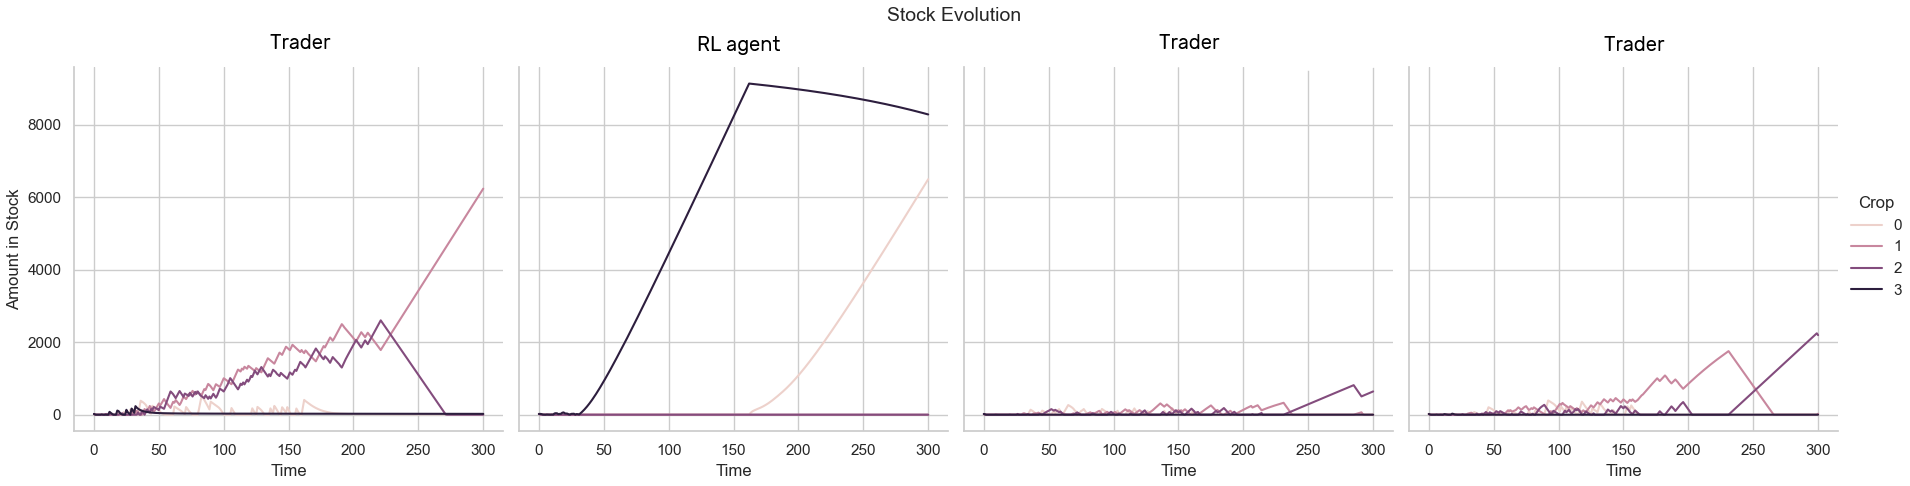
\includegraphics[width = 1\textwidth]{Figures/stock evolution.PNG}
    \caption{Stock evolution for the three \texttt{Trader} agents and the RL agent.}
    \label{fig:stock evolve}
\end{figure}





%command to display code:
%\begin{lstlisting}
%\end{lstlisting}
\newpage
\subsection{Outlook}
The current state of this project allows the pursuit of many directions. Especially with regards to machine learning a multitude of different scenarios could be simulated.

One example is a possible drought scenario. The current code can be easily extended to simulate time-varying water availability scenarios for the river. Thus it would be possible to train the agents to meet a certain demand threshold in each time step while the water availability is reduced. Such a scenario might yield interesting results where the agents have to cooperate, since there is a strong first-mover advantage for farmers that are further up the stream of the river.

Other directions would be to include more realistic agricultural models and processes in order to evaluate agricultural policies, implement more realistic agent personalities, refine the market model, apply the model to other markets with different commodities. Moreover, a game-theoretic analysis of our model might give another interesting perspective. Some of these features are partially or fully implemented already, but could not be adequately tested due to the lack of time.


Since this is our first project with machine learning, the development of the environment and algorithms took relatively long. Hyperparameter tuning of the PPO model would most likely improve the performance of the ML model a lot. Also, maybe there are other, better performing RL algorithms than PPO. For example, we found, that random sampling of the action space outperforms the Introverts almost always. Thus, maybe an algorithm with more drastic changes than PPO, which is designed to only alter the current policy relatively slowly, might be better performing.  

%\subsubsection{FAO-based crop model}
%The main income of farmers of this area is considered to be from agricultural activity and as the studied area is considered a semi-arid region, finding a water allocation scheme for a multi-crop cultivation pattern is of great importance. The annual agricultural benefit for the multi-crop cultivation pattern can be obtained as follow:

%\begin{equation}
%    \sum_{c=1}^{n} P^c \cdot A_t^c \cdot Y_t^c- C^c \cdot A_t^c= AB_t
%\end{equation}

%Here, \(AB_t\) is the annual benefit, \(P^c\) is unit benefit price per crop, \(A_t^c\) shows the area under cultivation for each crop for year t (ha),  \(C^c\) is the unit cost of producing each crop and n is the number of crops. \(Y_t^c\) denotes each crop yield under the deficit irrigation for year t (kg/ha). \(Y_t^c\) 


%\subsection{Global Warming Potential (GWP)}
%Agricultural activities are one of the main sources of greenhouse gas (GHG) emissions. GWP is an indicator that can reveal the severity of GHG emissions of agricultural activities and it is measured in CO2 equivalent. The goal of this study is to minimize the GWP. The total GWP (kg CO2-eq ha1) is consisting of GHG emissions from farming practices including fertilizers, biocide (herbicide, insecticide, and fungicide), machinery practices (farm tillage), and electricity consumption for irrigation. The total GWP can be calculated as follow:
%\begin{equation}
    %GWP_{t}=GWP_{fertilizer}+GWP_{biocide}+GWP_{machinery}+GWP_{electricity}  
%\end{equation}
                     
%\(GWP_{fertilizer}\) is defined as:
%\begin{equation}
%\begin{split}
%GWP_{fertilizer}=Organic fertilizer(manure) N rate(kg/ha)\cdot(0.8\%*1\%+3\% )*298 \\
%+Chemical fertilizer N rate(kg/ha)*8.3+P_2 O_5 rate(kg/ha)*1.50+K_2 O(kg/ha)*0.98 
%\end{split}
%\end{equation}


 

       
%Here 3\% and 0.8\% indicate N2O and NH3 emission factors, respectively. These factors are considered for broilers’ manure. Also, the value 298 represents the N2O factor for the 100-year time horizon. The N2O volatile rate is included by 1\% .  For the chemical fertilizers, manufacturing and transportation are included in the CO2-eq emissions factors. \(GWP_{biocide}\) can be calculated as:
%\begin{equation}
%GWP_{biocide}=Herbicide(kg/ha)*6.3+Insecticide(kg/ha)*5.1+Fungicide(kg/ha)*3.9                    \end{equation}                                                                            
%\(GWP_{machinery}\) is defined as:
%\begin{equation}
    %GWP_{machinery}=Machinery(MJ/ha)*0.071+Dissel Fuel(ltr/ha)*2.76 
%\end{equation}
%The \(GWP_{electricity}\) that is associated with irrigation can be determined as follow:
%\begin{equation}
    %GWP_{electricity}=Electricity(kWh/ha)*0.608 
%\end{equation}



\newpage
\bibliographystyle{ieeetr} 
\bibliography{AgentBasedModelling.bib}

\end{document}
